\documentclass{article}
\usepackage{graphicx} % Required for inserting images
\usepackage{amsmath}
\usepackage{booktabs}
\usepackage[margin=1in]{geometry}


\title{A Numerical Comparison of Linear Regression and Neural Networks as Parameter Estimators for the Dixon-Coles Model.}
\author{Aleksandr Beliaev}
\date{June 2026}

\begin{document}

\maketitle

\section{Introduction}

The purpose of this project is to compare a linear regression approach to an MLP for parameter estimation for a Dixon-Coles model. I take a feature set of elo, recent goal difference estimates, and team quality features sourced from FIFA/FC player ratings to estimate $\lambda_{away}, \lambda_{home}, \rho$ -- Dixon-Coles parameters. I present a within-noise difference in accuracy for the MLP ($RPS = 0.1756$) compared to linear regression ($RPS = 0.1762$) on test data.

This single-match edge, however, is misleading. The MLP is \emph{unstable} and generalizes poorly out of sample: small architecture changes swing its predictions dramatically, and it extrapolates catastrophically on unusual inputs. Concretely, when simulating the 2026 World Cup, widening the network from $64$ to $256$ hidden units moved the favourite from Spain to Germany ($22.4\%$ champion probability); and before a data fix, a team with a sparse player-ratings record (Egypt) was assigned a $65\%$ title probability. The linear Dixon-Coles estimator, by contrast, produces stable, bookmaker-like forecasts. The thesis of this report is therefore that near-identical aggregate accuracy hides a large gap in robustness in favour of the simpler, structured ``human'' model.

\section{Dixon-Coles Model}

The Dixon-Coles model (Dixon and Coles, 1997) models the goals scored by the home and away sides as two Poisson random variables $X \sim \text{Poisson}(\lambda_{home})$ and $Y \sim \text{Poisson}(\lambda_{away})$. Independent Poissons alone misestimate the frequency of low-scoring results (notably draws), so Dixon and Coles introduce a dependence correction $\tau$ on the four lowest scorelines:
\[
P(X=x, Y=y) = \tau_{\lambda_{home},\lambda_{away}}(x,y;\rho)\, \frac{\lambda_{home}^{x}e^{-\lambda_{home}}}{x!}\,\frac{\lambda_{away}^{y}e^{-\lambda_{away}}}{y!},
\]
with
\[
\tau = \begin{cases}
1 - \lambda_{home}\lambda_{away}\rho & (x,y)=(0,0)\\
1 + \lambda_{home}\rho & (x,y)=(0,1)\\
1 + \lambda_{away}\rho & (x,y)=(1,0)\\
1 - \rho & (x,y)=(1,1)\\
1 & \text{otherwise.}
\end{cases}
\]
The single correlation parameter $\rho$ captures the dependence between the two scores at low totals; a negative $\rho$ raises the probability mass on draws relative to the independent-Poisson baseline. In our fits $\rho \approx -0.10$, consistent with the literature.

Figure~\ref{fig:joint} shows the resulting joint scoreline distribution for a concrete example -- a hypothetical Spain (home) versus France (away) tie, with the linear model's fitted rates $\lambda_{Spain}=1.71$ and $\lambda_{France}=1.40$. The probability mass concentrates on low scores, peaking around $1$--$1$ and $2$--$1$.

\begin{figure}[h!]
\centering
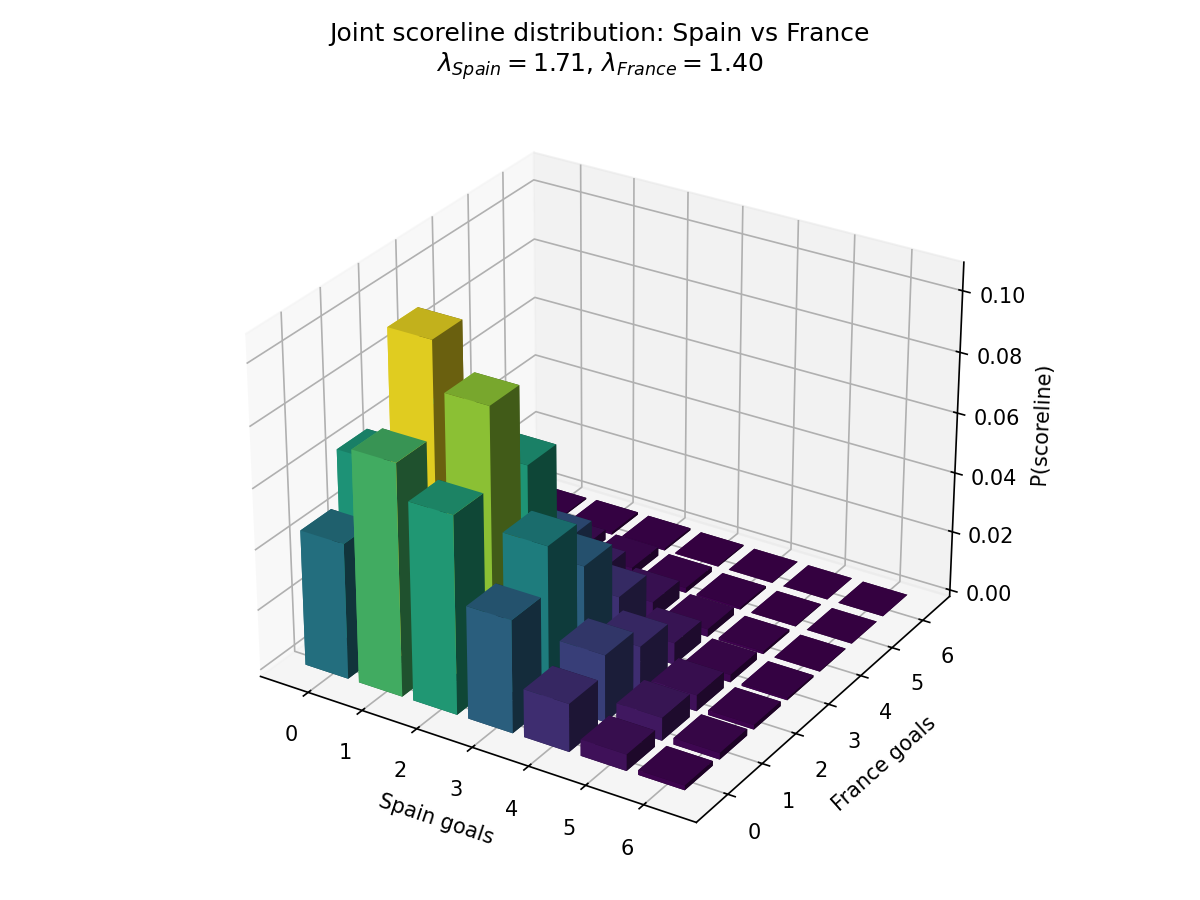
\includegraphics[width=0.75\textwidth]{figures/image.png}
\caption{Joint scoreline probability $P(X=x,Y=y)$ for Spain vs France, formed from the two
fitted Poisson rates. Height is the probability of each exact scoreline.}
\label{fig:joint}
\end{figure}

\section{Feature Set and Data}

\subsection{Match Results}

\textbf{Elo.} Each team carries an Elo rating updated after every match. The expected home score is
\[
E_{home} = \frac{1}{1 + 10^{(r_{away}-r_{home})/D}}, \qquad
r \leftarrow r + K\,(S - E),
\]
where $S\in\{1,\tfrac12,0\}$ is the realized result. Both the logistic divisor $D$ (default $800$) and the update rate $K$ are free parameters: $D$ controls how strongly a rating gap maps to a win probability, and $K$ how quickly ratings react to new results. We treat them as tunable and report a sensitivity study over $D \in \{200, 800, 1600\}$ with a fixed $K=50$ (Section~\ref{sec:elo}).

\textbf{Recent form.} Rather than a single goal-difference figure, we keep \emph{goals scored} and \emph{goals conceded} over each team's last ten matches as separate features. The hypothesis -- from football intuition rather than the data -- was that goals conceded would carry a stronger signal than goals scored, defensive solidity being a more stable team trait than finishing.

\subsection{FIFA (FC) Video Game}

Player ratings from the EA Sports FC (formerly FIFA) series are used as a proxy for squad quality, following prior work that built match-prediction features from grouped player ratings (Arntzen and Hvattum, 2021). % TODO: replace with the specific 2018 reference the author has in mind.
For each national team we take the top 25 players by overall rating and compute: the squad mean (\texttt{squad\_avg}); a dispersion term (\texttt{squad\_std}); positional means (\texttt{attack\_avg}, \texttt{midfield\_avg}, \texttt{defence\_avg}); a bench mean and dispersion for players ranked 12--25 (\texttt{bench\_avg}, \texttt{bench\_std}); and the best goalkeeper rating (\texttt{gk\_rating}). A secondary aim was exploratory: to see which of these features the models actually use, addressed in Section~\ref{sec:reduction}.

\section{Linear Regression}

The linear estimator fits two separate linear predictors over the (standardized) feature vector $\mathbf{x}$ and an intercept:
\[
\lambda_{home} = \boldsymbol\beta_h^\top [1,\mathbf{x}], \qquad
\lambda_{away} = \boldsymbol\beta_a^\top [1,\mathbf{x}],
\]
clipped to remain positive. The coefficients $\boldsymbol\beta_h,\boldsymbol\beta_a$ and the shared $\rho$ are estimated by maximum likelihood, propagating the predicted $\lambda$'s through the Dixon-Coles likelihood of Section 2 and minimizing the (temporal-decay weighted) negative log-likelihood with L-BFGS-B. A ridge penalty $\alpha\sum\beta^2$ on the slope coefficients is available.

A note on convexity: the Poisson negative log-likelihood is convex in the linear coefficients, but the $\tau(\rho)$ correction is bilinear in $(\rho, \lambda_{home}\lambda_{away})$, so once $\rho$ is estimated jointly the objective is no longer convex and a unique global optimum is no longer guaranteed. In practice the optimizer is well-behaved given a sensible initialization.

\section{Neural Network}

The neural estimator is a small multilayer perceptron: the 20-dimensional feature vector feeds a stack of fully connected ReLU layers (with dropout), and a final layer emits three values. The two goal rates are passed through a softplus to keep them positive, and $\rho$ through a $\tanh$ to constrain it to $[-1,1]$:
\[
\lambda_{home}, \lambda_{away} = \text{softplus}(\cdot), \qquad \rho = \tanh(\cdot).
\]
It is trained by mini-batch Adam on the same Dixon-Coles negative log-likelihood, with temporal-decay sample weights and early stopping on a validation split.

\section{Results}
\subsection{World Cup}

We simulate the 2026 World Cup $10{,}000$ times from each model's predicted goal rates, using the official bracket (group stage, eight best third-placed teams, full knockout tree). Treating matches as neutral, the linear model's championship probabilities are headed by Spain ($14.0\%$), France ($10.8\%$), Argentina ($8.6\%$), England ($7.6\%$) and Germany ($7.6\%$) -- a spread close to market expectations.

The MLP is far less stable. Under the validation-selected architecture (width $256$) it makes Germany a runaway favourite at $22.4\%$, while undervaluing France ($3.2\%$) and Argentina ($1.2\%$); under a narrower network (width $64$) Spain instead leads. We return to this instability in Section~\ref{sec:sweep}.

A natural final prediction is the ensemble that simply averages the two models' probabilities, combining the linear model's robustness with the MLP's non-linear mapping. Its leading championship probabilities are Germany ($15.0\%$), Spain ($14.7\%$), France ($7.0\%$), England ($6.8\%$), the Netherlands and Brazil ($6.1\%$); the per-team ensemble figures are reported alongside the individual models.  

\subsubsection{Draws in Play-Off's}

Knockout ties are decided by penalty shootouts, which are close to a coin flip but disproportionately influenced by the goalkeeper. We therefore resolve a tied knockout in favour of team $A$ with probability $\mathrm{gk}_A/(\mathrm{gk}_A+\mathrm{gk}_B)$, using the squad goalkeeper rating, rather than by overall strength $\lambda_A/(\lambda_A+\lambda_B)$. Because goalkeeper ratings vary less than overall strength, this compresses the favourites' shootout edge and improves underdog chances. The mean shift in championship probability is small ($0.23$pp for the linear model, $0.48$pp for the MLP) but systematic: Spain loses $2.0$pp (linear) and $5.2$pp (MLP), redistributed to weaker sides.

\subsection{MLP vs Linear Regression}

On the held-out test set (matches from October 2025 onward, including the World Cup window), the two models are effectively tied and both far ahead of a base-rate baseline ($RPS = 0.2234$): the MLP scores $RPS = 0.1756$ and the linear model $RPS = 0.1762$.

\subsubsection{Hyperparameter Sweep}
\label{sec:sweep}

For the linear model the only real hyperparameter is the ridge strength $\alpha$; validation favoured a light $\alpha = 10$, with performance degrading only for very large penalties ($\alpha = 10^4$). For the MLP we swept learning rate, depth, width and dropout ($55$ configurations). On single-match accuracy the architecture barely matters -- validation RPS spanned just $0.1866$--$0.1900$ across the entire grid.

The same insensitivity does \emph{not} hold for the downstream tournament forecast. As noted above, widening the network from $64$ to $256$ units changes the predicted World Cup favourite from Spain to Germany, even though both configurations have essentially identical test RPS. The MLP's tournament forecasts are thus unstable to architecture choices while the linear model's are robust. This is the core evidence for the report's thesis: equal single-match accuracy, but markedly worse generalization from the more flexible model.

\subsection{Non-linearity Problems}

Neural networks extrapolate poorly outside the training distribution. Several nations have sparse player-ratings records in FC26 (e.g. Egypt with $10$ rated players), which initially produced a zero bench average -- a value far outside the training range. The linear model absorbed this gracefully, but the MLP extrapolated it into a $65\%$ championship probability for Egypt. A linear fit is structurally incapable of this kind of blow-up; the neural network is acutely sensitive to it.

A related, more subtle symptom is that the MLP systematically undervalues South American sides (Argentina $1.2\%$, Brazil $4.8\%$) relative to both the linear model and bookmakers. The network appears to have latched onto a pattern that is not evidently present; both Argentina and Brazil are high elo (2nd and 4th) and high rated teams (3rd and 5th). Lacking interpretability, there is no straightforward way to confirm or correct it.

\subsection{Elo Sensitivity}
\label{sec:elo}

Re-deriving the Elo features with a fixed $K=50$ and divisor $D\in\{200,800,1600\}$ changed validation RPS only marginally. The flattest scale, $D=1600$, was best for both models (MLP $0.1860$, linear $0.1875$) versus the $D=800$ baseline (MLP $0.1866$, linear $0.1886$); the steep $D=200$ scale was marginally worst. Elo parameterization is a second-order effect here.

\subsection{Feature Reduction}
\label{sec:reduction}

Restricting the model to a ten-feature subset (Elo, bench average, a per-match goal difference, and attack/defence squad averages, home and away) cost almost nothing: linear RPS moved from $0.1880$ to $0.1890$ and MLP from $0.1866$ to $0.1888$. Half the feature set is therefore close to redundant -- the additional squad sub-features carry little independent signal, consistent with their high mutual correlation.

\subsection{Friendlies}

Dropping friendly matches from the training and validation sets hurt both models (linear $0.1881 \to 0.1921$, MLP $0.1866 \to 0.1893$). Two effects combine: friendlies are a large share of the data, so removing them shrinks the training set; and -- the more interesting football point -- friendlies are not pure noise, carrying real information about squad strength and form despite their lower stakes.

\subsection{Author's "Ball Knowledge"}

Having watched and played football for over a decade, I came into this project with assumptions about how different features would influence the $\lambda$ estimates. Because the linear model is interpretable, its fitted coefficients can be read directly; Table~\ref{tab:coef} lists the standardized home/away slope coefficients for the features discussed below.

Firstly, I split the usual goal difference into goals scored and goals conceded, expecting this to let the model distinguish attacking from defending sides. In the fit, both goals scored and goals conceded by either team raise goal expectation -- the lone exception being goals scored by the away team, which lowers the home team's expectation. This indicates that high-scoring teams tend both to score and to concede more, and vice versa.

Secondly, and more strongly, I believed that goals conceded would carry a better signal than goals scored. This held: the conceded coefficients are almost double the scored coefficients, suggesting that how much a team lets in says more about it than how much it puts away.

Thirdly, I expected a higher midfield average (more creative play) to raise goals and a higher defence average to lower them. The first held only weakly -- a highly rated midfield raised the home team's expected goals, but barely. The second was reversed: a strong defence \emph{increased} expected goals, and by more than midfield did. This suggests that a solid defence lets the rest of the team push higher up the pitch and attack with more players and more security, echoing analyses of Neuer's sweeper-keeper role at the 2014 World Cup (P. Vipond, 2014).

Fourthly, and most strikingly, the opposition's ranking matters more than one's own. The away team's Elo enters the home goal rate at $-0.213$, nearly three times the magnitude of the home team's own Elo ($+0.072$): who you face suppresses your scoring far more than your own quality lifts it.

Finally, against my pre-tournament favourite picks of France, Spain and Portugal: the simulated linear odds agree on Spain (1st) and France (2nd), but rate Portugal only 7th ($6.6\%$). The MLP is more and less sympathetic to Portugal -- a width-64 network put it at $8.7\%$, but the chosen width-64 network puts it at $2.1\%$. Perhaps we both see something there that the squad averages and elo alone miss.

\begin{table}[h!]
\centering
\small
\begin{tabular}{@{}lrr@{}}
\toprule
Feature & $\beta_{home}$ & $\beta_{away}$ \\
\midrule
intercept              & $+1.499$ & $+1.056$ \\
\midrule
home\_elo              & $+0.072$ & $-0.090$ \\
away\_elo              & $-0.213$ & $+0.109$ \\
home\_scored\_last10   & $+0.066$ & $+0.038$ \\
home\_conceded\_last10 & $+0.083$ & $+0.101$ \\
away\_scored\_last10   & $-0.031$ & $+0.049$ \\
away\_conceded\_last10 & $+0.027$ & $+0.006$ \\
home\_midfield\_avg    & $+0.061$ & $-0.050$ \\
home\_defence\_avg     & $+0.128$ & $-0.085$ \\
\midrule
\multicolumn{3}{l}{$\rho = -0.098$} \\
\bottomrule
\end{tabular}
\caption{Fitted standardized coefficients of the linear Dixon-Coles model (ridge $\alpha=10$),
for the features discussed in this section.}
\label{tab:coef}
\end{table}

\section{Future Steps}
%- A neutral-venue retrain. Right now home advantage lives in the intercept (1.499 vs 1.056), and I average both orientations to neutralize WC matches. Cleaner: add an explicit neutral flag as a feature so the model learns the home effect rather than us cancelling it post-hoc. Probably improves WC realism.
%- Ensemble the two models for the actual WC bet — average linear and MLP probabilities. Ensembling a robust + a flexible model usually beats either, and it'd damp the MLP's  Germany/South-America weirdness.
% Quantify "instability" properly. Right now it's anecdotal (Spain→Germany). You could train the MLP across N seeds × M architectures and report the variance of each team's championship probability vs the linear model's — turning the thesis into a hard number.
\subsection{Non-Constant WC Team Features}
Currently team features are frozen at the beginning of the world cup and all matches - from group stage to final - are computed with the same feature vector for a team. 
Varying the vector depending on the earlier results can introduce a more up-to-date feature assessement. Additionally, features can be increased lighter or stronger depending on the in-tournament performance. 

\subsection{Quantifying MLP 
Instability}

Right now the MLP instability is anecdotal (Spain→Germany). A sweep training the MLP across N seeds × M
architectures would allow us to report the variance of each team's championship probability vs the linear model's — turning a set of examples into a measurable quantity.

\subsection{Copula over $\rho$ and Negative Binomial Distributions.}

The Dixon-Coles $\tau$ correction is a low-order patch on the independence assumption, acting only on the four lowest scorelines. A more principled treatment would replace it with an explicit copula coupling the two marginal Poisson (or negative-binomial) counts, with $\rho$ becoming the copula's dependence parameter. This would model score dependence across the whole table rather than only at $0$ and $1$ goals, while still reducing 
to independent margins at $\rho = 0$.
Additionally, we can model goals scored with a Negative Binomial instead of Poisson. Football scores are mildly over-dispersed; and a Negative Binomial margin (one extra parameter) often beats Poisson.

\subsection{LSTM Representation Learning}

A more ambitious direction is to learn a team representation rather than hand-engineer one. An encoder would map per-match features to a latent vector $z_t$, and a recurrent state $c_t$ would integrate these over time -- internalizing a team's long-run state while still updating sharply when something material happens (a manager change, a key injury). Crucially, one could encode how much individual stars contribute (via xG and similar) so that the presence or absence of key players is reflected in $c_t$.

To make $z_t$ informative, the encoder would be trained by contrastive learning -- real fixtures against random match-ups -- and, more strongly, by a fully conditional objective that predicts $z_{t+k}$ from $c_t$ (maximizing the likelihood of the realized future state, potentially with an $L^2$ rather than purely cosine objective). The trained $c_t$ vectors would then replace the hand-built features as input to either the MLP or the linear Dixon-Coles model.

\begin{thebibliography}{9}
\bibitem{dixoncoles} M.~J. Dixon and S.~G. Coles (1997). Modelling Association Football Scores and Inefficiencies in the Football Betting Market. \textit{Journal of the Royal Statistical Society: Series C (Applied Statistics)}, 46(2), 265--280.
\bibitem{arntzen} H.~Arntzen and L.~M. Hvattum (2021). Predicting match outcomes in association football using team ratings and player ratings. \textit{Statistical Modelling}, 21(5).
\bibitem{thesefootballtimes} P.~Vipond (2014). How Manuel Neuer, Germany's 11th man, is revolutionising goalkeeping. \textit{These Football Times}.
\end{thebibliography}

\end{document}
